\section{Proposed system}

The proposed design for Wondough Bank's service can be seen in figure \ref{fullDesign}. The website sub-component may be seen in greater detail in figure \ref{website}. 

\begin{figure}
    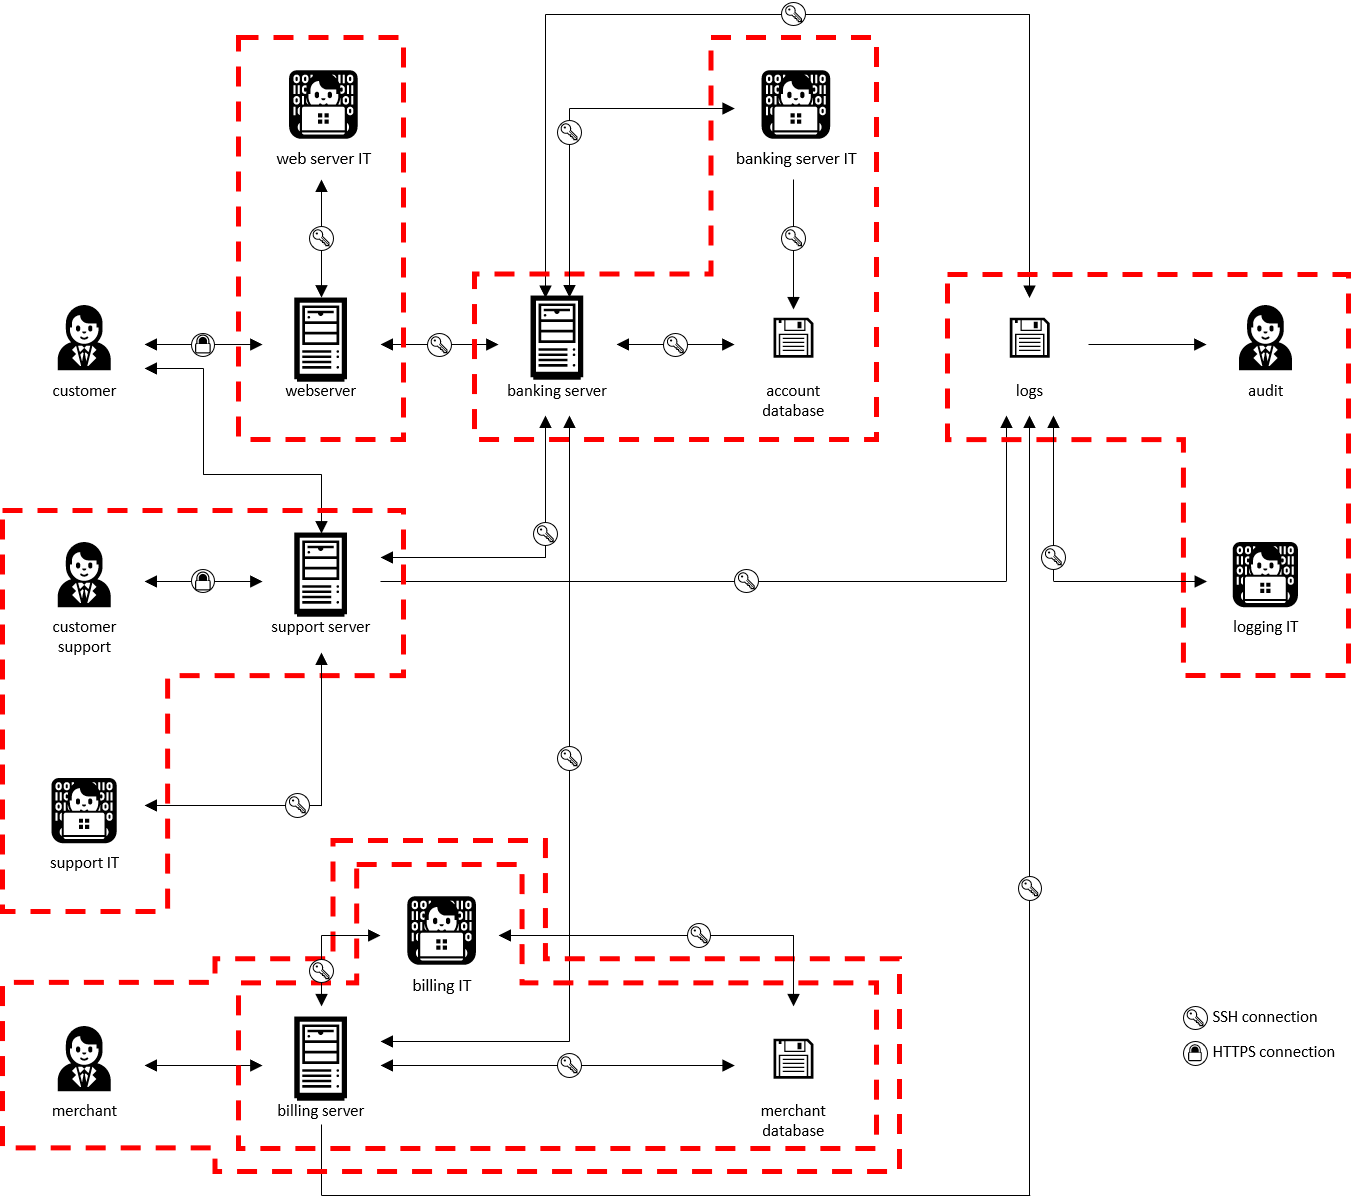
\includegraphics[width=\columnwidth]{images/bank-design}
    \caption{The proposed design for Wondough Bank's service}
    \centering
    \label{fullDesign}
\end{figure}

Connections marked with a key represent connections secured via SSH, while connections marked with a padlock represent connections secured via HTTPS. Unmarked connections assume an unsecured data channel. Red dashed boxes represent trust boundaries. 

The system generally aims to compartmentalise the system as much as possible. This provides additional security, as any attacks involving more than one server require the penetration of at least one trust boundary. 

\begin{figure}
    
\includegraphics[width=\columnwidth]{images/web-design}
    \caption{A more specific design for the bank's web-facing component}
    \centering
    \label{website}
\end{figure}

\subsection{Security measures}

There are a number of slightly unique or novel security measures in the proposed system design. The following section attempts to explain how they work and the justification behind them.

\subsubsection{Customer support verification}

One common attack vector for bank customers is impersonating a member of customer support. Similarly, a member of customer support could potentially “go rogue” and attack a customer's account.

While many consider phonelines to be a safe method of communication, “vishing” or “voice phishing” is on the rise. \cite{bbcPhone} \cite{bbcSmishing} Phone number spoofing can make an illegitimate call appear to be from a legitimate source. Holding open a line\footnote{
    During a landline phone call, depending on the network's configuration, a line may be kept open after a receiver has hung up. For a short window of time, future calls they make will reuse the same line to the original caller. \cite{conArtists}
} can redirect a call from a customer to their bank towards an attacker.

Such techniques mean that verification of both Wondough Bank's staff members and customers is necessary in every situation. The proposed system to satisfy such a goal is displayed in figure \ref{customerSupport}.

\begin{figure}
    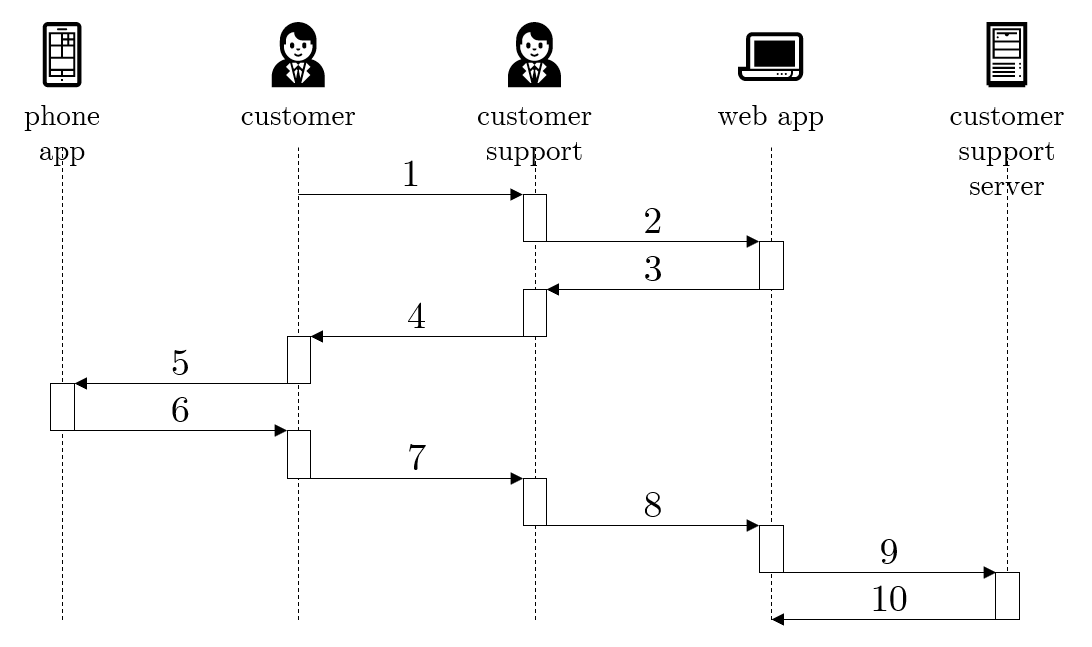
\includegraphics[width=\columnwidth]{images/customer-support}
    \caption{customer support verification}
    \centering
    \label{customerSupport}
\end{figure}

First, a customer contacts a member of customer support through a potentially insecure connection, such as a phone call. Alternatively, a member of customer support may contact the customer first. (step 1 on diagram)

To authenticate to the customer, the staff member's customer service terminal will provide a one-time access code (OTAC) generated from the time, the staff member's credentials, and the customer's credentials. The staff member passes this to a customer, who verifies it using the Wondough Bank phone app. (steps 2-5 on diagram)

After verifying the customer support member's OTAC, the phone app will provide a customer's own OTAC. They must then provide this to the customer support representative. (step 6-8)

The customer service web application will send both OTACs to the customer support server, which will verify the codes server-side, before granting the staff member access to the customer's account.

Such a system requires authorisation and consent from both the staff member and the customer before any changes to a customer's account may be made.

\subsubsection{Transaction integrity}

In order to guarantee the integrity of all transactions in the database, anapproach similar to Bitcoin's blockchain \cite{blockchain} will be used.

Every transaction will contain a hash made up of its own contents, the previous transaction's hash, and a random nonce. This nonce will be chosen so that the hash is in a specific form. For example, requiring the hash to start with a certain number of zeros. In order for a transaction to be accepted by the database, the hash field will be re-calculated on insertion, and verified for formatting. The formatting required may be changed in order to vary the amount of work required to calculate one hash.

In order for a malicious party to alter a previous transaction, they would have to re-calculate every hash between the altered entry and the most recent entry. Recalculation would need to be performed at a rate greater than that of transactions incoming to the bank. Therefore, in order to maliciously altery the contents of any transactions in the banking system, an attacker would require more total computing power than Wondough Bank owns. While initially Wondough Bank may be a small scale operation, as they grow, this will be harder and harder to achieve.

\subsubsection{Merchant authorisation}

Preventing a third party impersonating a merchanting is a similarly high priority requirement.  The proposed method for a merchant billing a customer's account is shown in Figure \ref{merchantBilling}.

\begin{figure}
    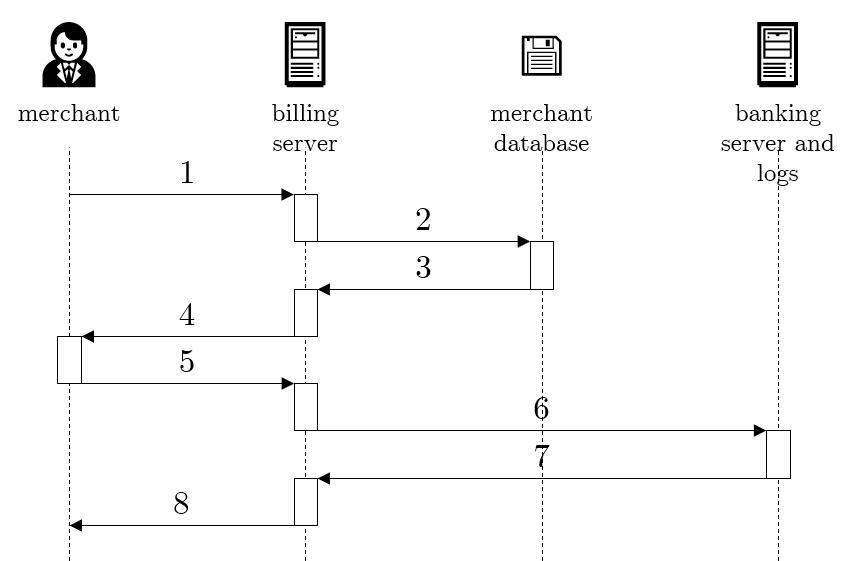
\includegraphics[width=\columnwidth]{images/merchant-billing}
    \caption{merchant billing customer's account}
    \centering
    \label{merchantBilling}
\end{figure}

To be accepted as a merchant, a third party must go through a verification process, during which they will be assigned a secret key, and an identifying name (IN). Since every merchant is assigned a unique secret key, damage if one such key is discovered is mitigated.

Upon connecting to the billing server, a merchant will supply their IN, a timestamp for the transaction, and a hash of their message encrypted with their secret key (message authentication code, MAC). The timestamp will prevent a replay attack from being performed, while the MAC will prevent an attacker simply changing the timestamp. (step 1)

When receiving their initial communication, the billing server will reference the merchant database for a secret key matching the IN provided. If one is not found, the whole communication is rejected. Otherwise, it is used to decrypt the MAC and verify the integrity and origin\footnote{
    While MACs do not normally provide non-repudiation in this way, each secret key is unique to a single merchant, and thus may be used to identify one. 
} of the message. (step 2, 3)

Future traffic sent across the network is encrypted with the merchant's secret key, providing secrecy. The billing server responds to the merchant, accepting the request, and the merchant replies with a billing for a customer. (step 4, 5) The transaction is sent to the banking server, and the communication is logged. (step 6)

If the whole process is successful, the banking server will reply to the billing server that the transaction was successful, which will forward the message to the merchant. (step 7, 8)

\subsection{Threat model}

There are a wide variety of possible attacks upon the proposed Wondough bank system. The STRIDE system was used to provide a threat model.

\subsubsection{Spoofing}

\begin{numbered}
    \item \label{impersonateAudit} Impersonate audit
    \begin{numbered}
        \item Gain access to logs
        \item Reconstruct customer's bank information from transaction history
    \end{numbered}
    
    \item \label{impersonateCustomerSupport} Impersonate customer support.
    \begin{numbered}
        \item Gain access to a customer's account
        \item Change a customer's details
        \item Access a customer's details to commit identity fraud
        \item Convince a customer to move money out of their account
    \end{numbered}

    \item \label{impersonateMerchant} Impersonate a merchant
    \begin{numbered}
        \item Bill customers incorrectly
    \end{numbered}

    \item \label{impersonateIt} Impersonate IT in any trust boundary
    \begin{numbered}
        \item May provide direct access to servers or databases
    \end{numbered}

    \item \label{impersonateWebserver} Impersonate the webserver or the support server
    \begin{numbered}
        \item Genuine users could connect to them mistakenly, allowing credentials to be stolen
        \item Could forge requests to other servers
    \end{numbered}
\end{numbered}

\subsubsection{Tampering}

\begin{numbered}[resume]

    \item \label{tamperAccountDatabase} IT could change account database without permission

    \item \label{tamperMerchantDatabase} IT could change merchant database without permission
    \begin{numbered}
        \item Allow arbitrary authorisation of merchants
        \item Allow arbitrary de-authorisation of merchants
    \end{numbered}

    \item \label{tamperSupportTickets} IT could alter support tickets
    \begin{numbered}
        \item Create fake tickets to waste staff time
        \item Alter/delete tickets to cause customer dis-satisfaction
    \end{numbered}
\end{numbered}

\subsubsection{Repudiation}

\begin{numbered}[resume]
    \item \label{repudiationFraud} The customer pretends to be the victim of fraud
    \begin{numbered}
        \item The bank must cover assets lost by fraud
    \end{numbered}

    \item \label{repudiationIt} Malicious activity by IT staff
    \item \label{repudiationCustomerSupport} Malicious activity by customer support
\end{numbered}

\subsubsection{Information disclosure}

\begin{numbered}[resume]
    \item \label{disclosureCustomerSupport} Malicious access to a customer's account by member of customer support
    
    \item \label{disclosureItDetails} A member of IT successfully attacks the account database, revealing a customer's information

    \item \label{disclosureItKeys} A member of IT accesses any of the keys used for encryption
\end{numbered}

\subsubsection{Denial of service}

\begin{numbered}[resume]
    \item \label{dosWebsite} DoS attack on website
    \item \label{dosCustomerSupport} DoS attack on customer support service
    \item \label{dosBillingServer} DoS attack on billing server
    \item \label{dosBankingServer} DoS attack on banking server
    \item \label{dosLogs} DoS attack on logs
\end{numbered}

\subsubsection{Elevation of privilege}

\begin{numbered}[resume]
    \item \label{eopXss} XSS attack using website
    \item \label{eopSqlInjection} SQL Injection using website registration form
    \item \label{eopCustomerSupport} XSS attack or SQL injection using customer support software
    \item \label{eopValidationDifference} Different servers could validate data differently when sending data to be logged – if some paths give different results, an attacker could exploit this
    \item \label{eopClientSideValidation} An attacker could bypass client-side validation and send un-validated information to a server
\end{numbered}

\subsection{Threat solution and evaluation}

\begin{longtable}{|| p{0.2\textwidth} | p{0.8\textwidth} ||}
    \hline
    Threat & Solution \\
    \hline\hline

              \ref{impersonateAudit} & 
        It is assumed for the purposes of this design that any system involving legislation-mandated auditors will be able to provide sufficient authentication.
    \\ \hline \ref{impersonateCustomerSupport} & 
        Customer support will be required to log in using two-factor authentication. They are authenticated to the user via a one-time access code.
    \\ \hline \ref{impersonateMerchant} &
        Upon an initial connection, a merchant is required to provide their Identifying Name, which is used to fetch a corresponding secret key from the database. All future traffic between parties is encrypted using this secret key.
    \\ \hline \ref{impersonateIt} &
        IT staff must undergo two-factor authentication before connecting to the database. A possible method to secure this attack surface further is to issue IT staff employee cards and card readers. Similarly to a home-banking card reader, these could provide a one time login code for the IT member.
    \\ \hline \ref{impersonateWebserver} &
        All webserver connections will be secured using HTTPS, providing a digital certificate.
    \\ \hline \ref{tamperAccountDatabase} \ref{tamperMerchantDatabase} &
        Only other servers will be given editing permissions for databases.
    \\ \hline \ref{tamperSupportTickets} &
        Write access to support tickets will be restricted to servers only. 
    \\ \hline \ref{repudiationFraud} &
        All connections to the webserver are made via HTTPS, thus removing the possibility of man-in-the-middle fraud. All log-ins to the website require two-factor authentication. All customer support changes require a code provided by the customer themselves.
    \\ \hline \ref{repudiationIt} \ref{repudiationCustomerSupport} &
        All staff members must access the server through secure channels such as SSH or HTTPS using two-factor authentication, guaranteeing non-repudiation. 
    \\ \hline \ref{disclosureCustomerSupport} &
        Customer support staff do not have the necessary access permissions to even access a customer's account details, without the customer first providing them with their account ID and a one-time password.
    \\ \hline \ref{disclosureItDetails} \ref{disclosureItKeys} &
        The database will be encrypted, and neceessary keys for decryption will be stored on HSMs, secured from IT staff.
    \\ \hline \textcolor{red}{\ref{dosWebsite}} &
        This is a possible weakness in the proposed design. No attempt was made in the design to mitigate denial of service attacks.

        A possible solution would be to track the IP address of incoming users, and deny access through the use of a firewall to users who make too many requests in too short of a length of time. However, this would still not stop bot-net attacks using many different IP addresses, or IP spoofing, which would rely on a solution at the ISP level.
    \\ \hline \textcolor{red}{\ref{dosCustomerSupport}} &
        Similarly, a full solution to DoS attacks on the customer support website is impossible as the service exists in the current design.

        One possible solution would be to host the customer support service on an intranet, blocking outside traffic. Denial of service attacks would only be possible from within the Wondough Bank organisation itself.
    \\ \hline \ref{dosBillingServer} &
        The billing server will be internal to Wondough Bank, so external DoS attacks will be impossible. 
    \\ \hline \ref{dosBankingServer} &
        All banking server requests with an invalid Identifying Name, timestamp or MAC will be rejected immediately.
    \\ \hline \textcolor{red}{\ref{dosLogs}} &
        This is a possible flaw in the system's design. For example, deliberately failing to log in repeatedly would write a lot of data to the logging system. Since this data is encrypted, this could be an expensive operation, and effectively perform a DoS attack on the logging server.

        A possible solution would be to distribute the logging server over a number of machines. Each machine would have a local cache, used to store frequent logs. This logs could be grouped together, before beging written to the central logging server in one transaction, minimising load.

        This solution would also remove the single point of failure in the system that is the logging server.
    \\ \hline \ref{eopXss} &
        All data stored from a user's input can be escaped before writing it to a web page, thus preventing a cross site scripting attack. The website may be written without JavaScript, allowing it to be disabled on the page as an extra layer of security.
    \\ \hline \ref{eopSqlInjection} &
        All actions in web-server will involve prepared statements, which automatically escape input data, preventing SQL injection.
    \\ \hline \ref{eopCustomerSupport} &
        This solution can be solved in a similar manner to that of \ref{eopXss} and \ref{eopSqlInjection}.
    \\ \hline \ref{eopValidationDifference} & 
        All validation occurs when data is first input to the system, meaning that only one, centralised validation check is necessary.
    \\ \hline \ref{eopClientSideValidation} &
        The system does not rely on any form of client-side validation.
    \\ \hline

\end{longtable}

\subsection{Legal and economic considerations}

There are a number of other considerations which must be considered for the design of the Wondough banking system. While legal requirements are perhaps the most obvious, and regulations are effectively mandatory, economic constraints on the system must also be considered.

\subsubsection{Legal requirements}

While there are many legal requirements for a business such as Wondough Bank, arguably the most important two are the UK's Data Protection Act from 1998 \ref{dataProtectionAct}, and the EU's General Data Protection Regulation, which will come in to force in 2018 \ref{generalDataProtectionRegulation}. 

The Data Protect Act states that data must be kept securely. As a banking application, security requirements are higher than for the general case web serice that The Data Protection Act was written for, so meeting these would not be a concern. However, the act states that data cannot be transmitted outside the European Economic Area without adequate protection. If Wondough Bank were to host their website using a cloud service, it may be necessary to ensure any data sent outside of the country was done so with adequate protection.

The EU's General Data Protecion Regulation is similar to the Data Protection Act, but provides more rights to a service's customers. For example, the act mandates that all data breaches are announced within 72 hours. The Wondough Bank system must be design in such a way that such breaches can be detected and reported on quickly and efficiently to stay within the bounds of the law.

\subsubsection{Economic constraints}

A system which fully meets or exceeds all requirements may still be prohibitively expensive for a small scale, start-up company like Wondough Bank to deploy, and thus may be unrealistic. It is necessary to consider the compromises which have to be made when designing such a system. 

Firstly, the choice of server host is important. While larger banks are able to afford their own dedicated servers for online banking, it may be necessary for a company on the scale of Wondough Bank to turn to a cloud-based hosting service such as Amazon Web Services or Microsoft Azure. While an in-house hosting solution may be cheaper in the long run, an organisation such as Wondough Bank may be unable to meet the necessary up-front expenditure.

However, hosting Wondough Bank's web-app in the cloud has some key advantages. Firstly, while the organisation is currently small, their intended scope for expansion is large. This is an area in which cloud services excel, and Wondough would need only to pay for any increased usage. If Wondough Bank were to install their own hosting infrastructure, they may find future expansion or upgrades costly.

Also, many hosts are willing to accept a large part of the responsibility for the security of data transmitted and stored on their servers. This means that Wondough Bank's resources may be focused more in other areas, and allows them to transfer risk to third parties. However, this may be disadvantageous, and Wondough Bank may want to be certain exactly what level of security data is afforded - a task which could be difficult when dealing with a large hosting company.

In the interests of security, Hardware Security Modules (HSMs) would be advantageous for any implementation of a secure system. Fortunately, many hosting services provide support for storing keys and passwords on HSMs.

Finally, For an organisation such as Wondough Bank, software lisences may be expensive. For example, certain implementations of SQL can be highly-priced. However, similarly to HSMs, hosting services may offer a "pay-by-use" pricing system for such software, moving a single fixed cost to several smaller, variable ones.

